\documentclass[../main.tex]{subfiles}
\graphicspath{{figures/}{../figures/}}

\begin{document}
\vspace{36pt}
\begin{center}
  \zihao{2}
  \songti{
    \textbf{西安财经大学}

    \textbf{本科毕业论文(设计)独创性及知识产权声明}
  }
\end{center}
\vspace{24pt}

本人郑重声明:所呈交的毕业论文是本人在导师的指导下取得的成果,论文写作
严格遵循学术规范。对本论文的研究做出重要贡献的个人和集体,均已在文中以明确
方式标明。因本毕业论文引起的法律结果完全由本人承担。

本毕业论文成果归西安财经大学所有。

\vspace{0.7cm}
特此声明
\vspace{3cm}

\begin{flushright}
  % \begin{table}[H]
    % \centering
    \begin{tabular}{l}
      毕业论文签名: \hphantom{陈伯硕,,,,00}\\
      专业: \MyMajor \\
      学号: \MyId \\
      \qquad 年 \quad 月 \quad 日 
    \end{tabular}
  % \end{table}
\end{flushright}

\officialDemand{
	\textbf{独创性及知识产权声明}
	\begin{officialDemandText}
		独创性及知识产权声明用以表明作者对于论文成果的独立研究及对论文知识产权的确认。
		每份论文的独创性及知识产权声明必须有作者的亲笔签名(或印章)和签名日期。
	\end{officialDemandText}
  \begin{officialDemandText}
    “西安财经大学本科毕业论文(设计)独创性及知识产权声明”用二号号宋体加粗居中,题
    前空三行,
    题后空二行打印内容,
    用小四号宋体。
    具体样式见模版。
  \end{officialDemandText}
}

% \includepdf{figures/statement.pdf}
% 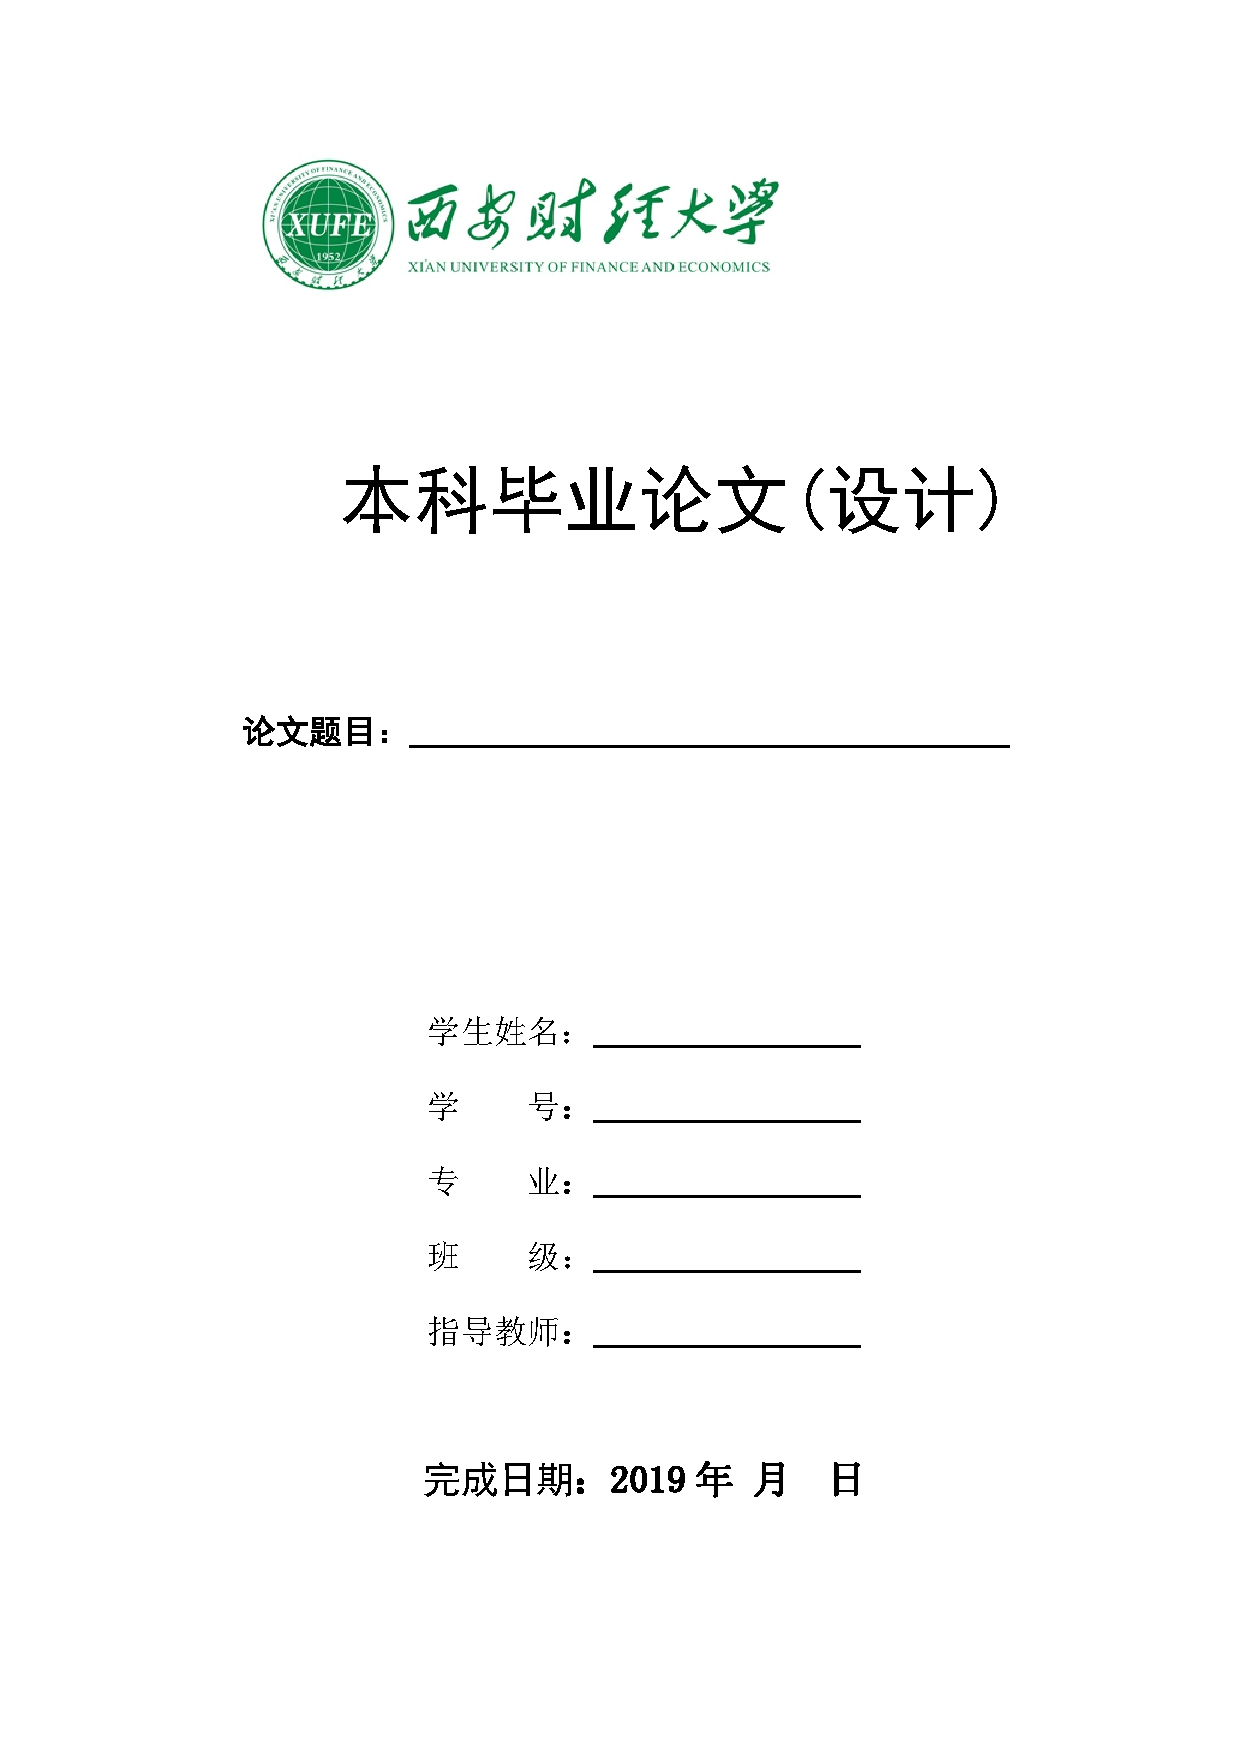
\includegraphics[pages={1}]{figures/cover.pdf}
% \includegraphics{figures/statement.pdf}

\newpage
\end{document}
